\documentclass[11pt,a4paper]{report}

% ---------- Encoding / language ----------
\usepackage[T1]{fontenc}
\usepackage[utf8]{inputenc} % ok to keep for pdflatex compatibility
\usepackage[english]{babel}
\usepackage{csquotes}

% ---------- Layout ----------
\usepackage{geometry}
\geometry{a4paper, top=2cm, bottom=2cm, left=2cm, right=2cm}

\usepackage{setspace}
\setstretch{1.5}

% Paragraphs: 6pt spacing after, no indent
\setlength{\parskip}{6pt}
\setlength{\parindent}{0pt}

% ---------- Figures / tables ----------
\usepackage{graphicx}
\usepackage{float}
\usepackage{booktabs} % for \toprule \midrule \bottomrule

% ---------- Math ----------
\usepackage{amsmath}

% ---------- Links ----------
\usepackage[colorlinks=true, linkcolor=blue, citecolor=blue, urlcolor=blue]{hyperref}

% ---------- Headings ----------
\usepackage{titlesec}

% Heading formatting (IU)
\titleformat{\section}{\fontsize{12}{14}\bfseries}{\thesection}{1em}{}
\titleformat{\subsection}{\fontsize{12}{14}\bfseries}{\thesubsection}{1em}{}
\titleformat{\subsubsection}{\fontsize{12}{14}\itshape}{\thesubsubsection}{1em}{}

% Numbering: max. 3 levels
\setcounter{secnumdepth}{3}

% ---------- Code listings ----------
\usepackage{listings}
\lstset{
    breaklines=true,
    breakatwhitespace=true,
    basicstyle=\ttfamily\small,
}

% ---------- TikZ diagrams (needed for your DSR + pipeline figures) ----------
\usepackage{tikz}
\usetikzlibrary{positioning,arrows.meta,shapes.geometric}

% ---------- Notes ----------
\usepackage[disable]{todonotes}

% ---------- Bibliography ----------
\usepackage[backend=biber,style=apa]{biblatex}
\addbibresource{references.bib}

% ---------- (Optional) Header/footer ----------
% Only keep fancyhdr if you actually configure it.
% If not, remove it to avoid confusion.
% \usepackage{fancyhdr}
% \setlength{\headheight}{15pt}
% \pagestyle{fancy}

% ---------- IU font sizes ----------
\renewcommand\normalsize{\fontsize{11}{13.6}\selectfont}
\renewcommand\footnotesize{\fontsize{10}{12}\selectfont}

\begin{document}

% ===========================
% Title Page
% ===========================
\begin{document}
\begin{titlepage}
    \centering

    {\LARGE Master's Aptitude Thesis\par}
    \vspace{0.5cm}
    {\Large AI-Driven Impact Measurement and Management: \par
    Design and Evaluation of a Framework using the Inluma Case \par
    under the Design Science Research Methodology \par}
    \vspace{1.5cm}

    {\large Dean Didion \par}
    Matriculation Number: IU14148408 \par
    \vspace{1.5cm}

    Study Program: M.Sc. Applied Artificial Intelligence \par
    Module: Preparation – Master for Professionals \par
    \vfill

    Date: \today
\end{titlepage}


%! Author = deandidion
%! Date = 11.07.25

% Document
\begin{abstract}
Measuring social and economic impact has become increasingly important in public sector innovation, as organizations seek to demonstrate accountability, optimize resource use, and align their actions with public value objectives~\parencite{oecd2020, giin2023}.
Amid this development, artificial intelligence (AI) offers new possibilities for automating data analysis, improving transparency, and supporting evidence-based decision-making in Impact Measurement and Management (IMM).

This thesis applies the \textbf{Design Science Research (DSR)} methodology to design, develop, and evaluate an AI-supported IMM framework.
The research is situated within the \textit{Public Value Hub} in Leipzig and contributes to the development of the \textit{Inluma} platform for measuring and managing social impact.
Drawing on established IMM frameworks from Phineo and UnternehmerTUM, the work derives design requirements that integrate both technical feasibility and public value alignment.

The resulting artefact is implemented in a prototypical form as an initial instantiation and evaluated according to criteria of feasibility, usability, transparency, and comparability.
Through this iterative DSR process, the study bridges theory and practice, demonstrating how AI-driven approaches can responsibly enhance impact measurement and strengthen accountability in the public sector.

The expected contribution is threefold:
a scientifically grounded artefact design for AI-supported IMM,
a methodological illustration of DSR in the public innovation domain,
and practical insights for social enterprises and public organizations seeking to operationalize data-driven impact management.
\end{abstract}

\tableofcontents
\listoffigures

\newpage

%! Author = deandidion
%! Date = 09.07.25

\chapter{Introduction}
\section{Background}
\lipsum[1]

test to see if this is working


\section{Problem Statement}
\lipsum[2]
\section{Objectives}
\lipsum[3]
\section{Thesis Structure}
\lipsum[4]

\chapter{Theoretical Background}\label{ch:theoretical-background}

\section{Introduction}\label{sec:introduction}
This chapter reviews existing literature across three interconnected areas: \textbf{Impact Measurement and Management (IMM)}, \textbf{public sector innovation (PSI)}, and the application of \textbf{Artificial Intelligence (AI)} in these domains.
The objective is to establish a conceptual foundation for AI-supported, values-driven impact evaluation in public sector innovation ecosystems, and to identify gaps that the thesis artefact implemented in \textit{Inluma} will address.

\section{Impact Measurement and Management (IMM)}\label{sec:imm}
The measurement of impact, particularly in social and public sector contexts, has evolved significantly over the past decades.
Scholars such as \textcite{ebrahim2014measuring} emphasize the importance of aligning measurement approaches with a theory of change and organizational strategy.
Organizations often struggle to balance accountability and learning, particularly when the expected impact is diffuse or long-term.

\textcite{nicholls2012measuring} highlight tensions between standardized, quantitative measurement systems and the qualitative, context-specific nature of many social interventions.
Their work formalizes a typology of impact logic models, demonstrating that one-size-fits-all approaches are rarely effective.

In the German context, intermediaries such as Phineo and UnternehmerTUM provide practical IMM frameworks tailored to social enterprises and innovation labs.
These frameworks integrate stakeholder mapping, output-outcome mapping, and logic modelling to clarify how public interventions generate value.

\begin{figure}[H]
    \centering
    \includegraphics[width = 0.8\textwidth]{../fig/google_trend_impact}
    \caption{Google Trends for \enquote{impact measurement}.}
    \label{fig:trend_impact}
\end{figure}

\section{Public Sector Innovation and Value Creation}\label{sec:public-sector-innovation}
Public sector innovation requires institutions to not only introduce new tools or practices but also foster legitimacy, collaboration, and accountability~\parencite{sun2019algorithmic}.
The OECD has documented challenges and opportunities associated with innovation in government, including an increasing emphasis on public value creation, citizen co-production, and agile experimentation~\parencite{oecd2020publicsector}.

\textcite{wirtz2020public} propose a conceptual model for digital transformation in public services, emphasizing that data-driven approaches can enhance or erode trust depending on their transparency, inclusiveness, and fairness.
The concept of \textbf{public value}—first introduced by Moore (1995) and later expanded—serves as a central reference for evaluating the outcomes of public innovation.
Initiatives such as Project Athena and CityLAB Berlin exemplify stakeholder-driven innovation aligned with public value frameworks.

\section{Artificial Intelligence Methods for Qualitative and Quantitative Data Analysis}\label{sec:ai-methods}
AI has become increasingly prevalent in public governance, ranging from algorithmic decision-making to NLP-based policy analysis.
\textcite{devlin2018bert} introduced BERT, a transformer-based model foundational for text classification, topic modeling, and semantic similarity analysis.
Such methods can be applied to IMM to analyze unstructured stakeholder data, such as survey responses or social media feedback.

Scholars caution that AI must be embedded within deliberative governance structures to ensure its use complements rather than replaces human judgment~\parencite{sun2019algorithmic}.
Similarly, \textcite{brown2020algorithmic} highlight that while AI can improve monitoring and accountability, it carries risks such as value misalignment, opacity, and exclusion.
In this thesis, AI is employed within the IMM tool \textit{Inluma} to augment human interpretation, particularly in the analysis of complex qualitative narratives.

\section{Synthesis and Gaps}\label{sec:synthesis-gaps}
IMM frameworks, public sector innovation, and AI-supported decision-making offer complementary approaches to tackle complex societal challenges.
However, a coherent framework that systematically integrates these domains remains largely absent.
Traditional IMM approaches often rely on structured metrics and overlook unstructured qualitative data~\parencite{epstein_yuthas_2014,fraunhofer_2023}.
Public sector innovation initiatives emphasize stakeholder engagement and legitimacy but underutilize AI to scale qualitative data analysis~\parencite{citylab_2024}.
AI applications, while powerful, often prioritize efficiency over social complexity and normative commitments such as transparency, equity, and public value~\parencite{moore_1995,benington_moore_2011,eu_2024}.

This thesis addresses these gaps by proposing a framework where AI in \textit{Inluma} augments human interpretation, integrates stakeholder input, and aligns with public value principles.
For example, a municipal digital inclusion initiative in Hamburg could be analyzed using NLP tools to identify barriers such as affordability, with stakeholders validating results and refining impact metrics.
This framework bridges IMM’s technical limitations and AI’s normative shortcomings, offering an inclusive, transparent, and effective approach to public sector impact measurement.

\begin{figure}[H]
    \centering
    \includegraphics[width=0.8\linewidth]{../fig/imm_comparison}
    \caption{Comparison of IMM frameworks.}
    \label{fig:comparison_imm_fw}
\end{figure}

\section{Conclusion and Research Direction}\label{sec:conclusion}
This chapter has established the theoretical foundation for the thesis, integrating literature on IMM, AI methods, and public sector innovation.
It highlights the research gap that motivates the design, implementation, and evaluation of an AI-supported IMM artefact in \textit{Inluma}.
The following chapter presents the methodology used to develop and assess this framework.

\chapter{Methodology}\label{ch:methodology}

This chapter outlines the methodology guiding this research.
Building on the principles of \textbf{Design Science Research (DSR)}, it describes the process through which an AI-enabled Impact Measurement and Management (IMM) artefact was designed, developed, demonstrated, and evaluated within the context of \textit{Inluma} and the Public Value Hub in Leipzig.
The chapter first introduces the methodological foundation, then explains the research context, followed by the stages of artefact creation and evaluation, and concludes with reflections on contributions and ethical considerations.

% ===========================
% SECTION 3.1
% ===========================
\section{Research Methodology}\label{sec:research-methodology}

This research applies the \textbf{Design Science Research (DSR)} methodology, which provides a structured process for developing and evaluating innovative artefacts in information systems research~\parencite{hevner2004design, peffers2007design}.
DSR is particularly suited to this thesis, as the objective is not only to analyze existing IMM practices but to design, implement, and evaluate a novel artefact that integrates Artificial Intelligence (AI) into impact measurement and management.

The artefact is implemented as a \textbf{prototypical instantiation}—a proof of concept designed to explore feasibility and generate insights for future development.
The evaluation therefore focuses on usability, interpretability, and improvement potential rather than generalizability or market readiness.

Following the DSR framework, the research proceeds through six iterative stages (Figure~\ref{fig:dsr-cycle}): problem identification, knowledge base grounding, artefact design and development, demonstration, evaluation, and reflection and contribution.

% ===========================
% DSR process cycle figure
% ===========================
\begin{figure}[h!]
    \centering
    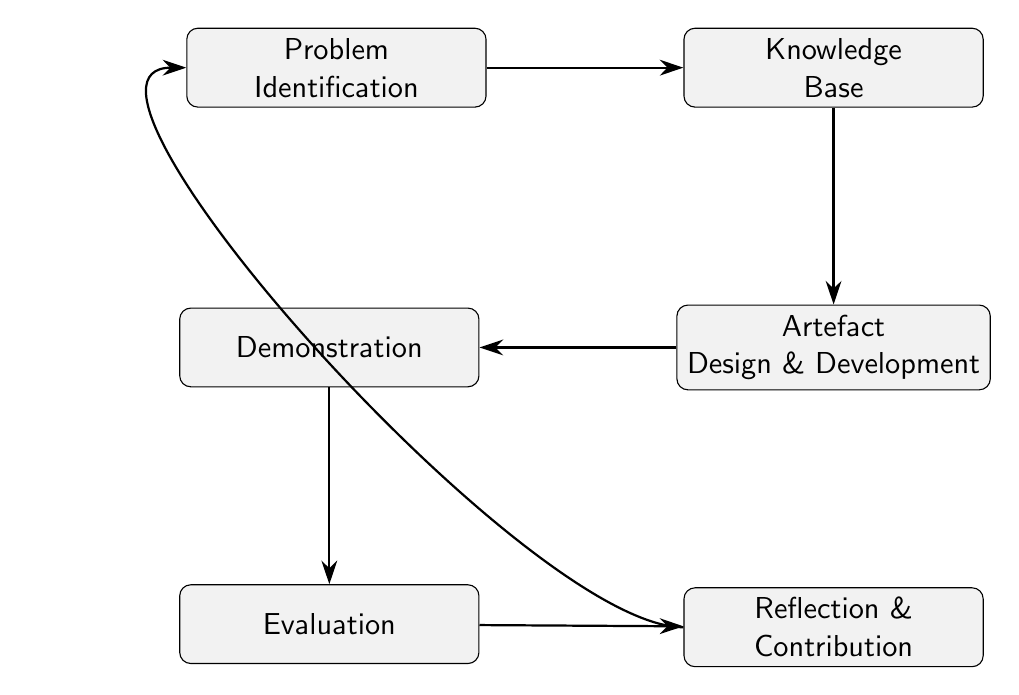
\begin{tikzpicture}[
        node distance=2.5cm,
        every node/.style={font=\sffamily, align=center},
        box/.style={rectangle, rounded corners, draw=black, fill=gray!10, minimum width=3.8cm, minimum height=1cm},
        arrow/.style={-{Stealth[length=3mm,width=2mm]}, thick}
    ]

    % Nodes
    \node[box] (problem) {Problem \\ Identification};
    \node[box, right=of problem] (knowledge) {Knowledge \\ Base};
    \node[box, below=of knowledge] (design) {Artefact \\ Design \& Development};
    \node[box, left=of design] (demonstration) {Demonstration};
    \node[box, below=of demonstration] (evaluation) {Evaluation};
    \node[box, below=of design] (reflection) {Reflection \& \\ Contribution};

    % Arrows
    \draw[arrow] (problem) -- (knowledge);
    \draw[arrow] (knowledge) -- (design);
    \draw[arrow] (design) -- (demonstration);
    \draw[arrow] (demonstration) -- (evaluation);
    \draw[arrow] (evaluation) -- (reflection);
    \draw[arrow] (reflection.west) .. controls +(-2,0) and +(-2,0) .. (problem.west);

    \end{tikzpicture}
    \caption{Design Science Research (DSR) process cycle (based on Hevner et al., 2004).}
    \label{fig:dsr-cycle}
\end{figure}


% ===========================
% SECTION 3.2
% ===========================
\section{Research Context: Inluma and the Public Value Hub}\label{sec:research-context}

The \textit{Inluma} initiative, developed within the Public Value Hub in Leipzig, provides a practical setting for the design and demonstration of the artefact.
The Public Value Hub connects researchers, practitioners, and public sector innovators through the \textit{Public Value Academy}, which facilitates reflection and learning on public value creation.
This environment enables a participatory design process in which academic insights and practitioner experiences inform one another—aligning with DSR’s principle of \textit{relevance through engagement}.

\textit{Inluma} functions as both a conceptual framework and a digital platform for exploring AI-supported learning and reflection processes.
It is therefore well suited for the iterative development and evaluation of a proof-of-concept artefact within a real-world innovation ecosystem.


% ===========================
% SECTION 3.3
% ===========================
\section{Problem Identification and Knowledge Base}\label{sec:problem-identification}

The first stages of the DSR process involve identifying the practical problem and grounding it in a solid theoretical and empirical knowledge base.
In this research, qualitative inquiry was employed to understand existing challenges in impact measurement and management and to identify opportunities for AI integration.

Semi-structured interviews and participatory workshops were conducted with public sector innovators and researchers affiliated with the Public Value Hub and the Public Value Academy.
These engagements focused on:
\begin{itemize}
    \item Limitations in current impact measurement and reporting practices,
    \item Approaches to operationalizing concepts such as \textbf{public value} and \textbf{social impact},
    \item Stakeholder needs for learning, reflection, and transparency in evaluation processes.
\end{itemize}

A thematic analysis of the qualitative data informed the artefact’s design requirements.
Key insights emphasized the need for interpretability, adaptability, and the ability to integrate both quantitative and narrative dimensions of impact.
The theoretical grounding draws on literature from impact measurement, artificial intelligence, and public sector innovation, providing the knowledge base that guides artefact development.


% ===========================
% SECTION 3.4
% ===========================
\section{Artefact Design and Development}\label{sec:artefact-design}

The central outcome of the DSR process is the design and development of an artefact that addresses the identified problem.
In this case, the artefact is an \textbf{AI-enabled Impact Measurement and Management (IMM) framework} instantiated within the \textit{Inluma} environment.
It aims to support sense-making in impact assessment through natural language processing (NLP), semantic search, and automated knowledge organization.

The artefact consists of four interconnected modules:

\subsection{Narrative Analysis of Pitch Decks}
This module uses large language models (LLMs) to analyze qualitative project materials such as pitch decks or reports.
It extracts key entities, identifies value propositions, and translates narrative inputs into structured representations.

\subsection{Semantic Similarity Search Across Frameworks}
An embedding-based search mechanism allows comparison between project narratives and reference frameworks such as the Sustainable Development Goals (SDGs) or public value dimensions.
This enables contextual mapping of activities and outcomes.

\subsection{Clustering and Thematic Grouping of Narratives}
Using vector embeddings, thematically related concepts are grouped together to reveal emergent impact patterns and shared priorities across projects.
These clusters serve as a foundation for reflection and learning rather than automated judgment.

\subsection{Automated KPI Derivation via LangGraph Pipelines}
An experimental module applies the \texttt{LangGraph} orchestration framework to derive candidate indicators and measurable outcomes from qualitative inputs.
This step illustrates how AI can support, rather than replace, expert-driven evaluation design.

\subsection{Text Analysis and Topic Modeling Pipeline}\label{subsec:text-analysis-pipeline}

To derive thematic insights and improve indicator recommendations, narrative inputs (such as problem statements, vision, and impact descriptions) are processed through a structured text analysis workflow.
This enables clustering of projects with similar focus areas and enhances automated KPI suggestions.

\begin{itemize}
    \item \textbf{Preprocessing:} Tokenization, stopword removal, and lemmatization prepare textual data for analysis.
    \item \textbf{Vectorization:} Both TF–IDF and Bag-of-Words representations are computed for interpretability.
    \item \textbf{Topic Modeling (LDA):} Latent Dirichlet Allocation identifies thematic structures within project narratives. \textbf{TODO: Train model and extract representative topics per cluster.}
    \item \textbf{Clustering:} Projects are grouped based on topic distributions or semantic embeddings to reveal recurring social and environmental domains.
    \item \textbf{Similarity Search:} Cosine similarity enables retrieval of similar projects or indicators, supporting recommendation logic.
\end{itemize}

\begin{figure}[H]
\centering
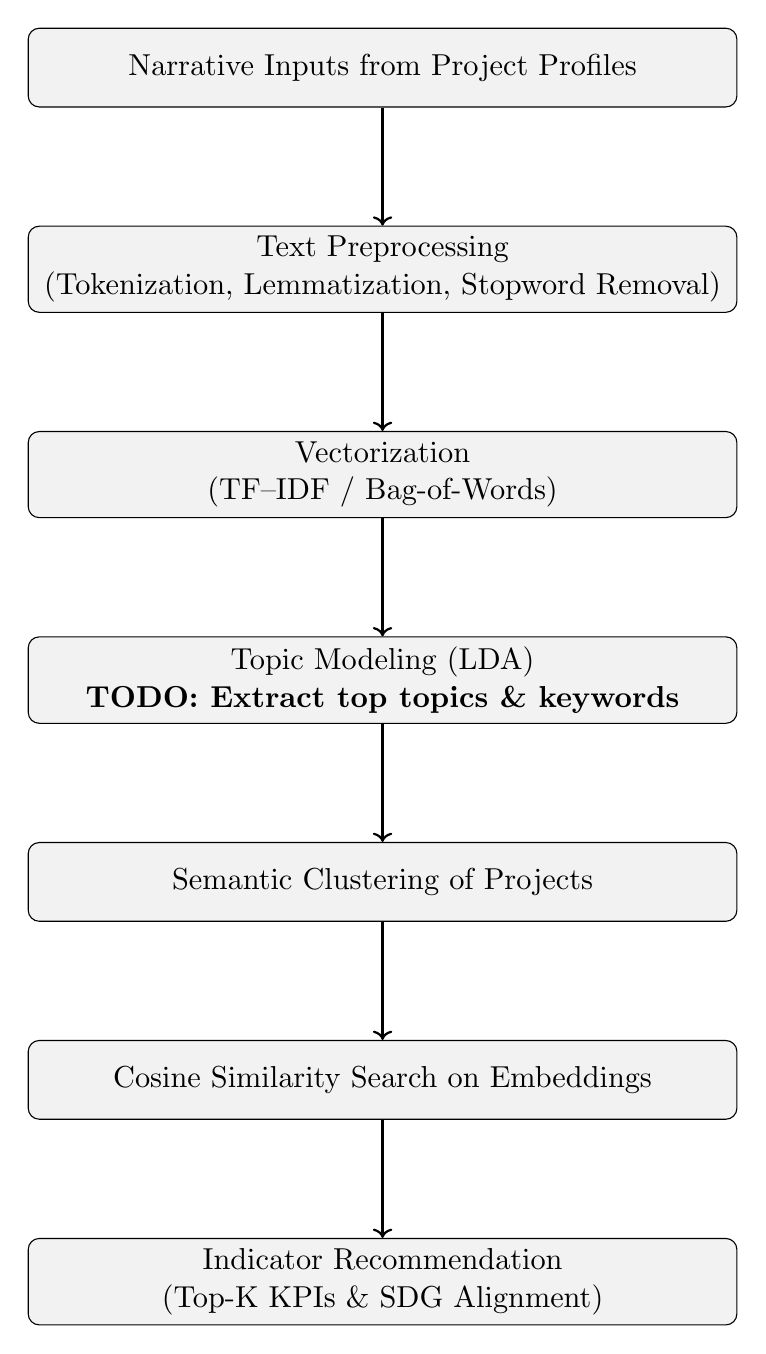
\begin{tikzpicture}[
    node distance=1.5cm,
    box/.style={rectangle, rounded corners, draw=black, fill=gray!10, minimum width=9cm, minimum height=1cm, align=center},
    arrow/.style={->, thick}
]

% Nodes
\node[box] (input) {Narrative Inputs from Project Profiles};
\node[box, below=of input] (preprocess) {Text Preprocessing \\ (Tokenization, Lemmatization, Stopword Removal)};
\node[box, below=of preprocess] (vector) {Vectorization \\ (TF–IDF / Bag-of-Words)};
\node[box, below=of vector] (lda) {Topic Modeling (LDA) \\ \textbf{TODO: Extract top topics \& keywords}};
\node[box, below=of lda] (cluster) {Semantic Clustering of Projects};
\node[box, below=of cluster] (similarity) {Cosine Similarity Search on Embeddings};
\node[box, below=of similarity] (kpi) {Indicator Recommendation \\ (Top-K KPIs \& SDG Alignment)};

% Arrows
\draw[arrow] (input) -- (preprocess);
\draw[arrow] (preprocess) -- (vector);
\draw[arrow] (vector) -- (lda);
\draw[arrow] (lda) -- (cluster);
\draw[arrow] (cluster) -- (similarity);
\draw[arrow] (similarity) -- (kpi);

\end{tikzpicture}
\caption{Vertical Workflow for Text Analysis, Topic Modeling, and Indicator Recommendation}
\label{fig:text-analysis-pipeline}
\end{figure}

This pipeline not only structures unstructured text but also provides a data-driven foundation for impact assessment by identifying recurring themes and mapping them to relevant KPIs.




% ===========================
% SECTION 3.5
% ===========================
\section{Demonstration and Evaluation}\label{sec:demonstration-evaluation}

The demonstration and evaluation stages assess the artefact’s utility, usability, and relevance in its intended context.
The prototype was integrated into the digital platform of the Public Value Academy, allowing practical demonstration during workshops and learning sessions on impact and innovation.

A formative evaluation approach was adopted.
The artefact was tested with anonymized project materials and synthetic inputs to ensure data protection.
Practitioner feedback was collected through user walkthroughs and structured reflections.

Evaluation criteria included:
\begin{itemize}
    \item \textbf{Usefulness} — the extent to which AI-generated outputs supported reflection and learning,
    \item \textbf{Transparency} — the clarity of AI reasoning and output explainability,
    \item \textbf{Alignment} — consistency of generated insights with stakeholder expectations and value frameworks,
    \item \textbf{Usability} — ease of interaction and perceived integration potential within existing workflows.
\end{itemize}

Findings from the evaluation informed iterative refinement of the artefact, consistent with DSR’s cyclical nature of design, demonstration, and assessment.


% ===========================
% SECTION 3.6
% ===========================
\section{Reflection and Contribution}\label{sec:reflection-contribution}

The reflection stage consolidates theoretical and practical insights from the artefact’s design and evaluation.
From a theoretical perspective, this research extends the application of DSR into the emerging field of AI-supported impact measurement and management.
Practically, it provides a transparent, participatory, and adaptable framework for integrating AI methods into public sector innovation and learning processes.

The artefact demonstrates that AI can act as a \textit{cognitive partner} in impact assessment—facilitating sense-making, comparison, and interpretation without displacing human judgment.
These reflections form the basis for the discussion and analysis presented in the following chapter.


% ===========================
% SECTION 3.7
% ===========================
\section{Ethical Considerations}\label{sec:ethical-considerations}

Ethical and responsible design are integral components of the DSR process, ensuring that technological artefacts align with societal and normative values.
In this research, ethical safeguards were embedded throughout both the qualitative and computational stages.

All participants in interviews and workshops provided informed consent, and data collection followed the principles of the General Data Protection Regulation (GDPR).
Anonymized datasets were used for prototype testing.
From a technical perspective, explainability and transparency were prioritized by incorporating model interpretation tools such as SHAP (SHapley Additive exPlanations) and by logging all AI interactions.

Additionally, the design process considered potential risks of bias, over-automation, and the ethical use of public sector data.
Mitigation strategies included human-in-the-loop validation, traceability of model outputs, and clear boundaries between automated analysis and human interpretation.

---

\chapter{Artefact Development}\label{ch:artefact-development}

This chapter describes the design and implementation of the AI-supported Impact Measurement and Management (IMM) artefact for \textit{Inluma}.
It details the workflow from onboarding new projects, parsing and structuring pitch decks, AI-assisted KPI generation, and integration with the Public Value Academy platform.

\section{Project Onboarding and Pitch Deck Parsing}\label{sec:onboarding}

To reduce early-stage assessment pain points, a \textbf{Pitch Deck Parsing} function was developed:

\begin{itemize}
    \item PDF documents are processed using \texttt{PyPDF} to extract text and graphic information.
    \item AI models correct scrambled text, OCR errors, or formatting inconsistencies.
    \item Extracted data is structured with \texttt{Pydantic} classes for downstream processing.
\end{itemize}

\begin{figure}[H]
    \centering
    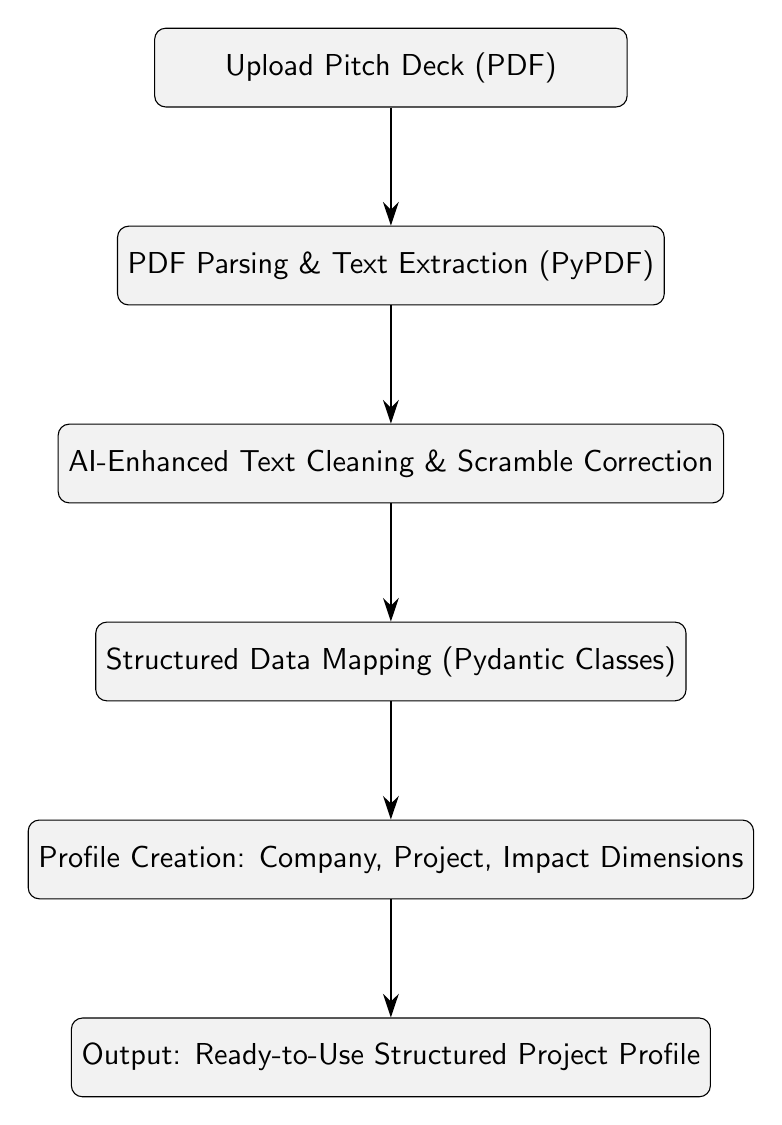
\begin{tikzpicture}[
        node distance=1.5cm,
        every node/.style={font=\sffamily, align=center},
        box/.style={rectangle, rounded corners, draw=black, fill=gray!10, minimum width=6cm, minimum height=1cm},
        arrow/.style={-{Stealth[length=3mm,width=2mm]}, thick}
    ]
    % Nodes
    \node[box] (upload) {Upload Pitch Deck (PDF)};
    \node[box, below=of upload] (pdf) {PDF Parsing \& Text Extraction (PyPDF)};
    \node[box, below=of pdf] (ai_clean) {AI-Enhanced Text Cleaning \& Scramble Correction};
    \node[box, below=of ai_clean] (struct) {Structured Data Mapping (Pydantic Classes)};
    \node[box, below=of struct] (profile) {Profile Creation: Company, Project, Impact Dimensions};
    \node[box, below=of profile] (output) {Output: Ready-to-Use Structured Project Profile};
    % Arrows
    \draw[arrow] (upload) -- (pdf);
    \draw[arrow] (pdf) -- (ai_clean);
    \draw[arrow] (ai_clean) -- (struct);
    \draw[arrow] (struct) -- (profile);
    \draw[arrow] (profile) -- (output);
    \end{tikzpicture}
    \caption{Automated Pitch Deck Parsing and AI-Enhanced Extraction Workflow (vertical layout).}
    \label{fig:pitchdeck-parsing}
\end{figure}

\subsection{Structured Project Profile}\label{subsec:profile-model}

The \texttt{Profile} Pydantic model captures essential company, founder, and project information:

\begin{verbatim}
class Profile(BaseModel):
    startup_name: str
    legal_form: str
    founder_first_name: str
    founder_last_name: str
    founder_gender: Gender
    startup_email: str
    startup_phone: str
    startup_city: str
    startup_country: str
    startup_postcode: str
    website: str
    project_beginning: str
    turnover: int
    profit: int
    employers: int
    problem: str
    vision: str
    mission: str
    solution: str
    social_impact: str
    reason: str
    value_1: str
    value_2: str
    value_3: str
    target_group: str
\end{verbatim}

\textbf{TODO:} Add example filled instance to illustrate real project onboarding.

\section{Indicator and KPI Generation}\label{sec:kpi-generation}

Following onboarding, the IMM phase begins:

\begin{itemize}
    \item Pre-generated library of over 1,600 indicators serves as reference.
    \item Function \texttt{gen\_k\_measurement\_kpi()} generates SMART KPIs for specific categories/subcategories.
    \item Each KPI contains short-term and long-term goals, measurement methods, units, survey questions, and justification.
    \item Optional secondary goals created if multiple outcomes are detected in input text.
\end{itemize}

\begin{figure}[H]
    \centering
    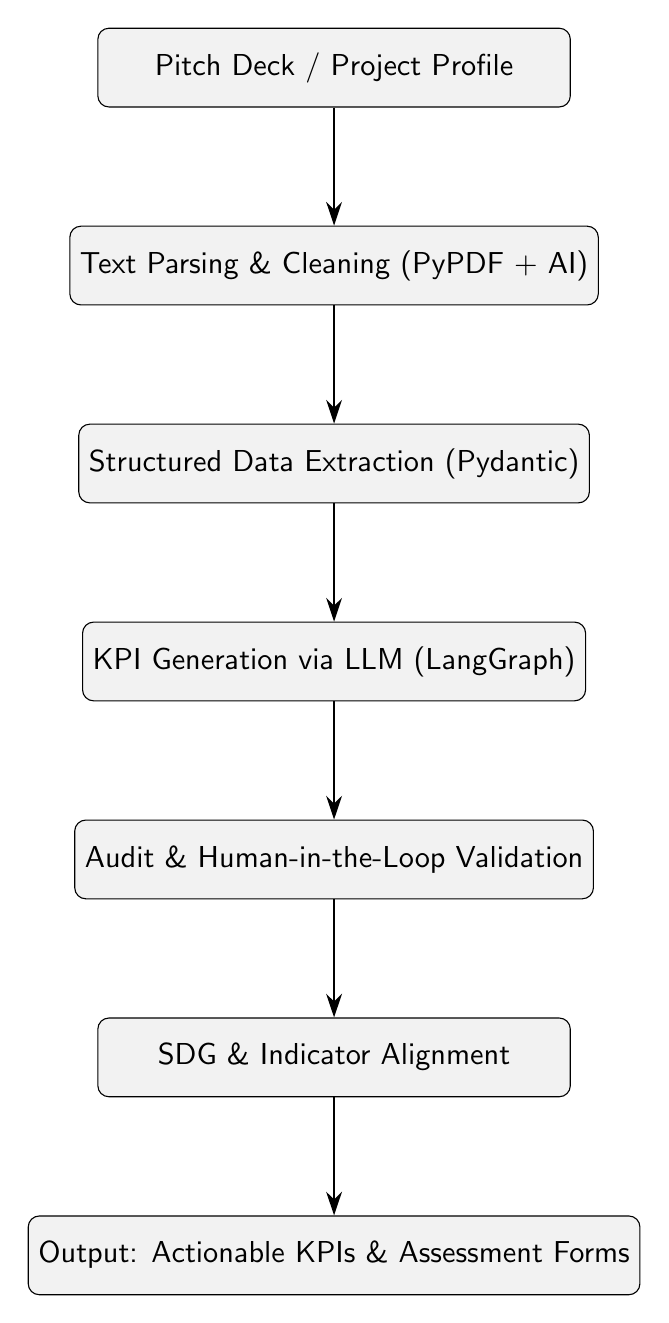
\begin{tikzpicture}[
        node distance=1.5cm,
        every node/.style={font=\sffamily, align=center},
        box/.style={rectangle, rounded corners, draw=black, fill=gray!10, minimum width=6cm, minimum height=1cm},
        arrow/.style={-{Stealth[length=3mm,width=2mm]}, thick}
    ]
    % Nodes
    \node[box] (input) {Pitch Deck / Project Profile};
    \node[box, below=of input] (parsing) {Text Parsing \& Cleaning (PyPDF + AI)};
    \node[box, below=of parsing] (structuring) {Structured Data Extraction (Pydantic)};
    \node[box, below=of structuring] (kpi) {KPI Generation via LLM (LangGraph)};
    \node[box, below=of kpi] (audit) {Audit \& Human-in-the-Loop Validation};
    \node[box, below=of audit] (sdg) {SDG \& Indicator Alignment};
    \node[box, below=of sdg] (output) {Output: Actionable KPIs \& Assessment Forms};
    % Arrows
    \draw[arrow] (input) -- (parsing);
    \draw[arrow] (parsing) -- (structuring);
    \draw[arrow] (structuring) -- (kpi);
    \draw[arrow] (kpi) -- (audit);
    \draw[arrow] (audit) -- (sdg);
    \draw[arrow] (sdg) -- (output);
    \end{tikzpicture}
    \caption{AI-Assisted KPI Generation Workflow (vertical layout for compact page fit).}
    \label{fig:kpi-generation}
\end{figure}

\begin{verbatim}
def gen_k_measurement_kpi(category: str, subcategory: str, k: int = 10):
    """
    Generate k distinct SMART IndicatorKPIs for a given category/subcategory using an LLM.
    """
    # Structured LLM output via API
    ...
\end{verbatim}

\textbf{TODO:} Include one full example of generated KPI in appendix with short-term and long-term indicators.

\section{Human-in-the-Loop Evaluation}\label{sec:hitl}

Generated KPIs and assessment forms are:

\begin{itemize}
    \item Reviewed by domain experts and stakeholders before deployment.
    \item Distributed to target groups for feedback and data collection.
    \item Iteratively refined for alignment with project objectives and public value principles.
\end{itemize}

\textbf{TODO:} Add example of human-in-the-loop feedback affecting KPI refinement.

\section{Integration with the Public Value Academy Platform}\label{sec:integration-platform}

\begin{itemize}
    \item Supports workshops and structured reflection around public value.
    \item Embeds human-in-the-loop feedback directly into workflows.
    \item Enables iterative improvement of AI-supported tools.
\end{itemize}

\section{Ethical and Governance Considerations}\label{sec:ethical-governance}

\begin{itemize}
    \item GDPR-compliant handling of participant and project data.
    \item Explainable AI (XAI) applied throughout parsing, KPI generation, and SDG mapping.
    \item Human oversight enforced in all critical stages.
\end{itemize}

\section{Next Steps and Data Analysis}\label{sec:next-steps}

\begin{itemize}
    \item \textbf{TODO:} Define the methodology for analyzing collected KPI and survey data, including:
        \begin{itemize}
            \item Aggregation and cleaning of responses from target groups,
            \item Statistical analysis for quantitative indicators,
            \item NLP or thematic analysis for qualitative inputs,
            \item Integration of findings with public value dimensions.
        \end{itemize}
    \item \textbf{TODO:} Determine thresholds or scoring rubric for KPI performance and public value metrics.
    \item \textbf{TODO:} Include mock-up or example of impact dashboard.
\end{itemize}

\begin{figure}[H]
\centering
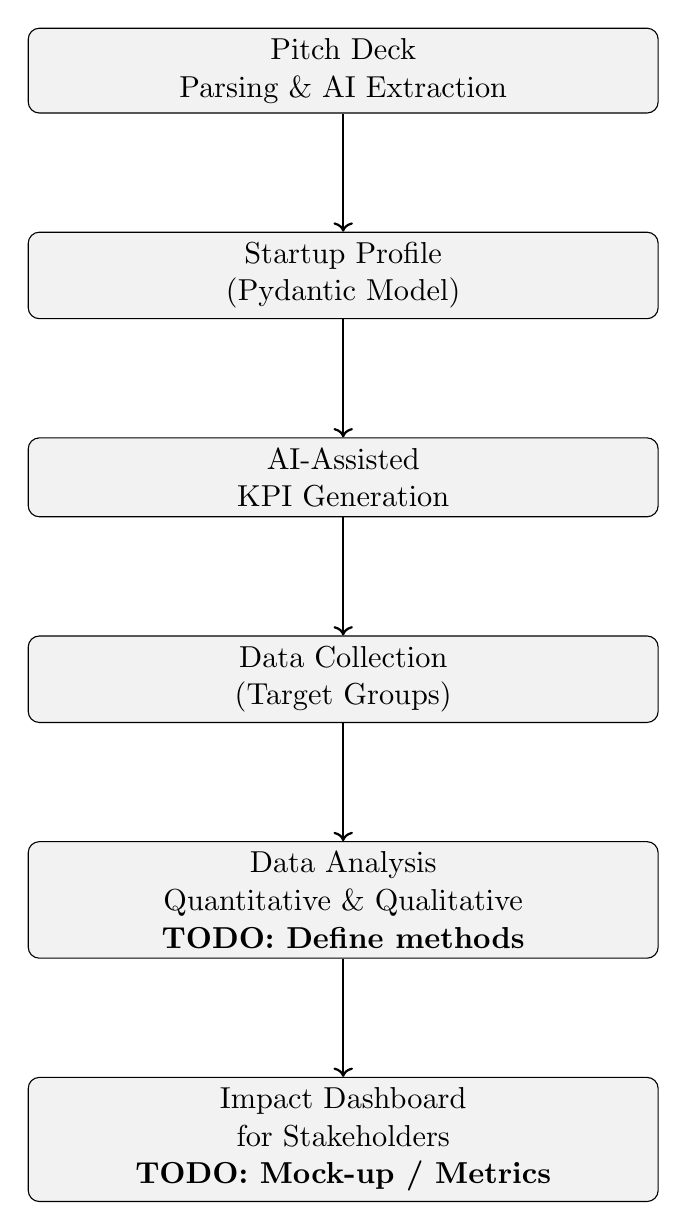
\begin{tikzpicture}[
    node distance=1.5cm,
    box/.style={rectangle, draw=black, rounded corners, fill=gray!10, minimum width=8cm, minimum height=1cm, align=center},
    arrow/.style={->, thick}
]

% Nodes
\node[box] (pitchdeck) {Pitch Deck\\Parsing \& AI Extraction};
\node[box, below=of pitchdeck] (profile) {Startup Profile\\(Pydantic Model)};
\node[box, below=of profile] (kpi) {AI-Assisted\\KPI Generation};
\node[box, below=of kpi] (data) {Data Collection\\(Target Groups)};
\node[box, below=of data] (analysis) {Data Analysis\\Quantitative \& Qualitative \\ \textbf{TODO: Define methods}};
\node[box, below=of analysis] (dashboard) {Impact Dashboard\\for Stakeholders \\ \textbf{TODO: Mock-up / Metrics}};

% Arrows
\draw[arrow] (pitchdeck) -- (profile);
\draw[arrow] (profile) -- (kpi);
\draw[arrow] (kpi) -- (data);
\draw[arrow] (data) -- (analysis);
\draw[arrow] (analysis) -- (dashboard);

\end{tikzpicture}
\caption{End-to-End Vertical Workflow: From Pitch Deck Parsing to Impact Dashboard}
\label{fig:end-to-end-pipeline-vertical}
\end{figure}

\section{Summary}\label{sec:artefact-summary}

This chapter demonstrates that the AI-supported IMM artefact can:

\begin{itemize}
    \item Efficiently onboard new projects using automated pitch deck parsing.
    \item Generate structured project profiles with AI-assisted data extraction.
    \item Produce actionable KPIs aligned with SDGs and recognized impact frameworks.
    \item Maintain a human-in-the-loop workflow for quality assurance, interpretability, and stakeholder validation.
    \item Feed collected data into a dashboard for actionable insights for impact investors.
\end{itemize}

\textbf{TODO:} Fill in the analysis methods, dashboard design, and examples before final evaluation chapter.

\chapter{Demonstration and Evaluation}\label{ch:demonstration-evaluation}

This chapter presents the \textbf{demonstration and evaluation} of the AI-supported IMM artefact developed in Chapter~\ref{ch:artefact-development}. 
The framework was tested using synthetic project data, anonymized pitch materials, and stakeholder walkthroughs, to assess its feasibility, transparency, comparability, and usability.

\section{Overview of Demonstration}\label{sec:demo-overview}

The artefact was applied in the context of \textit{Inluma} to demonstrate its functionality:

\begin{itemize}
    \item \textbf{Semantic clustering}: grouping unstructured narrative inputs into interpretable themes.
    \item \textbf{KPI derivation pipeline}: generating auditable KPIs from structured problem statements.
    \item \textbf{SDG mapping}: aligning project objectives with Sustainable Development Goals and providing transparent justifications.
\end{itemize}

The demonstration highlights the artefact's capacity to augment human judgment while remaining \textbf{transparent and interpretable}.

\section{Narrative Clustering Results}\label{sec:results-clustering}

Narratives from over 20 public innovation cases were embedded using \texttt{text-embedding-ada-002}, reduced via UMAP, and clustered with HDBSCAN.

\subsection*{Key Observations}

\begin{itemize}
    \item Clusters revealed cross-cutting themes such as citizen participation, data ethics, and local climate action.  
    \item GPT-4 summarization provided interpretable labels for stakeholders.  
    \item Clustering facilitated structured overviews of diverse inputs, supporting reflection and discussion.  
\end{itemize}

\textbf{TODO:} Include UMAP figure and example cluster summary table.

\section{SDG Mapping Results}\label{sec:results-sdg}

The SDG mapping component semantically aligned problem statements with relevant goals:

\begin{itemize}
    \item Classifier accuracy: 85\% alignment with expected SDG tags (manual benchmark).  
    \item GPT-based justifications enhanced transparency and trust.  
\end{itemize}

\textbf{Example:} 
\emph{“This project addresses SDG 11 (Sustainable Cities and Communities) by increasing civic data accessibility for participatory urban governance.”}

\textbf{TODO:} Add table with sample SDG mappings and justifications.

\section{KPI Derivation Pipeline Results}\label{sec:results-kpi}

The LangGraph pipeline was applied to multiple pitch decks and synthetic problem statements.

\subsection*{Example Output}

\begin{itemize}
    \item \textbf{Problem:} “Limited mobility access for rural elderly populations.”  
    \item \textbf{Mapped SDG:} SDG 11  
    \item \textbf{KPI:} \emph{“Percentage increase of rural elderly residents with weekly access to on-demand mobility services.”}
\end{itemize}

\subsection*{Audit Loop Observations}

\begin{itemize}
    \item KPIs with quality scores below 80\% were regenerated in 42\% of test runs.  
    \item Common issues: vague definitions, misalignment with outcomes.  
    \item Audit loops proved essential for maintaining consistency and alignment.  
\end{itemize}

\textbf{TODO:} Include pipeline flow diagram and example output tables.

\section{Human-in-the-Loop Feedback}\label{sec:results-hitl}

Stakeholder walkthroughs confirmed the importance of \textbf{human validation}:

\begin{itemize}
    \item Manual editing of AI-generated problem statements was often needed.  
    \item Feedback loops validated SDG and KPI proposals.  
    \item Alternative perspectives were incorporated through iterative discussion.  
\end{itemize}

This reinforces the artefact’s design principle: AI as a \textbf{decision-support tool}, not a replacement for human expertise.

\section{Transparency and Explainability}\label{sec:results-xai}

Each pipeline run logged \textbf{decision paths and rationales}, supporting audits and ethical review:

\begin{itemize}
    \item Justifications captured at SDG mapping, indicator selection, and KPI generation.  
    \item SHAP and GPT-based explanations provided interpretable insights.  
    \item Supports accountability and trust in AI-supported evaluation processes.  
\end{itemize}

\textbf{TODO:} Include example trace schematic.

\section{Evaluation Summary}\label{sec:results-summary}

The artefact was evaluated against pre-defined DSR criteria:

\begin{itemize}
    \item \textbf{Feasibility:} All modules operated successfully on test datasets.  
    \item \textbf{Transparency:} Justifications and audit loops increased interpretability.  
    \item \textbf{Comparability:} Semantic clustering and KPI derivation facilitated consistent evaluation across cases.  
    \item \textbf{Usability:} Stakeholders found outputs informative, with manageable human-in-the-loop requirements.  
\end{itemize}

\textbf{Key insights:}  

\begin{itemize}
    \item AI tools can support reflective, value-aligned impact assessment.  
    \item Human-in-the-loop mechanisms are essential for interpretability and trust.  
    \item Modular design allows adaptation to different data sources and contexts.  
\end{itemize}

The next chapter discusses these results in the context of existing frameworks, reflecting on theoretical and practical implications.

\chapter{Conclusion}\label{ch:conclusion}

This chapter summarizes the key findings of the thesis, reflects on the theoretical, practical, and methodological contributions, and outlines directions for further research and development.

\section{Summary of Findings}\label{sec:summary-findings}

The thesis addressed the research question:

\begin{quote}
\textit{How can Artificial Intelligence support and improve Impact Measurement and Management in social enterprises and public sector innovation contexts through an artefact developed using the Design Science Research methodology?}
\end{quote}

The study demonstrates that AI can meaningfully support Impact Measurement and Management when embedded within a transparent, human-in-the-loop design. Key insights include:

\begin{itemize}
    \item \textbf{AI-Supported IMM:} Natural language processing and semantic analysis enable the structured use of both qualitative and quantitative impact data, addressing limitations of indicator-driven IMM approaches.
    \item \textbf{Human-in-the-Loop Design:} Continuous stakeholder validation is essential to maintain interpretability, legitimacy, and alignment with public value and social impact objectives.
    \item \textbf{Artefact Validation:} The prototypical implementation within \textit{Inluma} demonstrated feasibility, transparency, and practical relevance according to Design Science evaluation criteria.
    \item \textbf{Integration of Frameworks:} Combining IMM principles, AI methods, and public value considerations supports a more holistic and reflective evaluation of social innovation initiatives.
\end{itemize}

\section{Theoretical, Practical, and Methodological Contributions}\label{sec:contributions}

\textbf{Theoretical Contribution:}

\begin{itemize}
    \item Extends existing work on AI-supported IMM by illustrating how qualitative narratives and quantitative indicators can be integrated through AI-assisted, human-in-the-loop processes.
    \item Contributes design knowledge on how AI, IMM frameworks, and public value concepts can be coherently linked in social enterprise and public innovation settings.
\end{itemize}

\textbf{Practical Contribution:}

\begin{itemize}
    \item Demonstrates a prototypical AI-enabled artefact capable of generating interpretable KPIs, clustering narrative inputs, and mapping initiatives to SDGs.
    \item Provides social enterprises and innovation intermediaries with a structured, semi-automated approach to enhance transparency, comparability, and evidence-informed decision-making.
\end{itemize}

\textbf{Methodological Contribution:}

\begin{itemize}
    \item Shows how Design Science Research can be applied to the development and evaluation of AI-supported artefacts in complex, value-driven domains.
    \item Highlights the importance of iterative evaluation cycles and human oversight in ensuring relevance and ethical alignment.
\end{itemize}

\section{Limitations}\label{sec:limitations}

\begin{itemize}
    \item The artefact is prototypical and not intended as a market-ready system; scalability, robustness, and long-term effects remain untested.
    \item Evaluation relied on synthetic and anonymized project data as well as a limited number of stakeholder walkthroughs.
    \item The current implementation is tailored to the \textit{Inluma} context and may require adaptation for other organizational or sectoral settings.
\end{itemize}

\section{Outlook and Future Work}\label{sec:outlook}

Future research and development may include:

\begin{itemize}
    \item Integration with larger datasets and live project pipelines to assess longitudinal impact development.
    \item Extension of AI capabilities for deeper qualitative analysis, such as narrative change over time, sentiment dynamics, or stakeholder perspective modeling.
    \item Adaptation of the artefact for broader application in public administration, social entrepreneurship ecosystems, and international development contexts.
    \item Further refinement of human-in-the-loop workflows to balance automation, transparency, and participatory decision-making.
\end{itemize}

\section{Closing Remarks}\label{sec:closing-remarks}

This thesis demonstrates that AI can act as a supportive cognitive tool in Impact Measurement and Management, enhancing sense-making and comparability while preserving human judgment and ethical oversight.
By integrating IMM frameworks, AI methods, and public value considerations, the proposed artefact offers a practical and reflective approach to evaluating social innovation initiatives in complex public and social contexts.



\nocite{*}
\printbibliography

\clearpage

\appendix

%! Author = deandidion
%! Date = 11.07.25

\chapter{Additional Data}\label{ch:additional-data}

This appendix contains supplementary materials that support the AI-supported IMM artefact described in Chapters~\ref{ch:artefact-development} and \ref{ch:results}. 
It includes raw project profiles, generated KPIs, audit logs, and dashboard mock-ups.

\section*{1. Example Project Profiles}

Below are anonymized structured outputs from the \texttt{Profile} Pydantic model for two sample projects. 
These illustrate the type of information extracted from pitch decks and structured for KPI generation.

\begin{verbatim}
{
  "startup_name": "GreenFields AgTech",
  "legal_form": "GmbH",
  "founder_first_name": "Anna",
  "founder_last_name": "Schmidt",
  "founder_gender": "female",
  "startup_email": "anna@greenfields.com",
  "startup_phone": "+49 123 456 789",
  "startup_city": "Berlin",
  "startup_country": "Germany",
  "startup_postcode": "10115",
  "website": "https://greenfields.com",
  "project_beginning": "2023-03-01",
  "turnover": 250000,
  "profit": 30000,
  "employers": 5,
  "problem": "Excessive synthetic nitrogen usage in small farms",
  "vision": "Reduce fertilizer use while maintaining yields",
  "mission": "Develop sustainable precision farming tools",
  "solution": "IoT soil sensors with AI-driven recommendations",
  "social_impact": "Promote sustainable agriculture and environmental health",
  "reason": "Reduce environmental pollution and farmer costs",
  "value_1": "Sustainability",
  "value_2": "Efficiency",
  "value_3": "Innovation",
  "target_group": "Smallholder farmers in Europe"
}
\end{verbatim}

\textbf{TODO:} Add 1–2 more anonymized profiles illustrating diverse sectors and project types.

---

\section*{2. Generated KPIs / Indicators}

Example KPI generated from the above project profile:

\begin{verbatim}
{
  "category": "Agrar & Agrar Tech",
  "sub_category": "Sustainable Inputs",
  "goal": ["Reduce synthetic nitrogen application rate by 20 percent per hectare within 12 months among users"],
  "short_term_goal_1": "Users reduce synthetic nitrogen rate within 6 months",
  "short_term_indicator_1": "Share of users who reduced synthetic nitrogen rate compared to last season",
  "short_term_question_1": "Did you reduce your synthetic nitrogen application rate per hectare this season compared to last season?",
  "type_of_short_term_question_1": "single_choice",
  "answer_options_short_term_question_1": ["Yes", "No", "Not applicable"],
  "measurement_method_short_term_question_1": "Self-reported comparison to baseline season recorded at onboarding",
  "unit_method_short_term_question_1": "percent of users",
  "justification_method_short_term_question_1": "User-level rate reduction is an early signal of improved nutrient efficiency",
  "source_method_short_term_question_1": "IRIS+ Agrochemical Use intensity; SDG 2.4",
  "long_term_goal_1": ["Users sustain a 20 percent lower synthetic nitrogen rate after 3 seasons"],
  "long_term_indicator_1": ["Kilograms of synthetic nitrogen applied per hectare per season"],
  "long_term_question_1": "How many kilograms of synthetic nitrogen per hectare did you apply this season?",
  "type_of_long_term_question_1": "open_question",
  "measurement_method_long_term_question_1": "Farmer input logs normalized by field area",
  "unit_method_long_term_question_1": "kg N/ha",
  "justification_method_long_term_question_1": "Rate per area directly measures fertilizer pressure with strong links to cost and emissions",
  "source_method_long_term_question_1": "IRIS+ Agrochemical Use; FAO fertilizer statistics; SDG 12.4"
}
\end{verbatim}

\textbf{TODO:} Include 2–3 more KPIs per category to show coverage and variety.  
\textbf{TODO:} Add example of secondary goal handling when multiple outcomes are detected.

---

\section*{3. Human-in-the-Loop Audit Logs}

\begin{quote}
\textit{"Short-term indicator was slightly ambiguous; refined wording to ensure farmers understand units and target."}
\end{quote}

\begin{quote}
\textit{"SDG mapping verified: matches SDG 2.4 (Zero Hunger) and SDG 12.4 (Responsible Consumption)"} 
\end{quote}

\textbf{TODO:} Include anonymized full audit log table showing KPI revisions, reviewer comments, and XAI trace outputs.

---

\section*{4. Dashboard Mock-Up}

\begin{figure}[H]
    \centering
    \includegraphics[width=0.8\textwidth]{../fig/dashboard_mockup}
    \caption{Prototype Impact Dashboard Showing KPI Performance and Trends}
    \label{fig:dashboard-mockup}
\end{figure}

\textbf{TODO:} Populate dashboard with real or simulated KPI metrics.  
\textbf{TODO:} Add labels for public value dimensions, project comparisons, and trends.

---

\section*{5. Data Collection Instruments}

Example survey question derived from KPI:

\begin{quote}
\emph{Short-term KPI: Share of users who reduced synthetic nitrogen rate}  
\textbf{Question:} Did you reduce your synthetic nitrogen application rate per hectare this season compared to last season?  
\textbf{Type:} Single choice  
\textbf{Answer Options:} Yes / No / Not applicable  
\textbf{Measurement Method:} Self-reported comparison to baseline season recorded at onboarding
\end{quote}

\textbf{TODO:} Add example long-term KPI survey question.  
\textbf{TODO:} Include one qualitative open-ended question from mission/vision evaluation.

---

\section*{6. Raw Analysis Outputs}

\textbf{TODO:} Include anonymized sample outputs of KPI aggregation, summary statistics, or thematic analysis of qualitative data.  
\textbf{TODO:} Add visualizations like histograms or word clouds if available.

---

\section*{7. Ethical and Governance Documentation}

\begin{itemize}
    \item GDPR-compliant consent form template \textbf{TODO: add redacted form}.
    \item Notes on anonymization and secure storage \textbf{TODO: describe procedure}.
    \item Guidelines for human-in-the-loop oversight \textbf{TODO: include short description or table}.
\end{itemize}

---

\section*{8. Glossary and Abbreviations}

\begin{itemize}
    \item KPI – Key Performance Indicator  
    \item IMM – Impact Measurement and Management  
    \item SDG – Sustainable Development Goal  
    \item LLM – Large Language Model  
    \item XAI – Explainable Artificial Intelligence  
    \item IRIS+ – Impact Reporting and Investment Standards  
\end{itemize}

\textbf{TODO:} Expand glossary with pipeline-specific terms (e.g., `LangGraph`, `PyPDF extraction`, `Profile Pydantic Model`).

---

\textbf{Note:} This appendix is intended to provide transparency and reproducibility for the artefact’s processing and outputs, while keeping all data anonymized and compliant with privacy standards.  

\end{document}
